\documentclass[10pt]{article}
\usepackage[a4paper,margin=1.5cm,top=1.2cm,bottom=1.4cm]{geometry}
\usepackage[T1]{fontenc}
\usepackage{mathptmx}
\usepackage{microtype}
\usepackage{graphicx}
\usepackage{booktabs}
\usepackage{tabularx}
\usepackage{array}
\usepackage{xcolor}
\usepackage{placeins}
\usepackage[font=footnotesize,labelfont=bf,skip=2pt]{caption}
\usepackage{enumitem}
\usepackage{titlesec}
\usepackage[hidelinks]{hyperref}
\titlespacing*{\section}{0pt}{5pt plus 1pt}{2pt}
\titleformat{\section}{\normalsize\bfseries}{\thesection}{0.5em}{}
\titlespacing*{\subsection}{0pt}{3pt}{1pt}
\titleformat{\subsection}{\small\bfseries}{\thesubsection}{0.5em}{}
\setlength{\parskip}{2pt}
\setlength{\parindent}{0pt}
\setlist{nosep,leftmargin=1.2em}
\setlength{\textfloatsep}{5pt plus 1pt}
\setlength{\floatsep}{4pt}
\setlength{\intextsep}{4pt}
\renewcommand{\arraystretch}{1.05}
\newcolumntype{Y}{>{\raggedright\arraybackslash}X}
\pagestyle{plain}
\begin{document}
\begin{center}
{\large\bfseries Logistic Regression vs.\ Gradient Boosting on an Anonymised Tabular Dataset}\\[2pt]
\textbf{Matric No.:} <MATRIC NO> \quad \textbf{Name:} <FULL NAME> \quad \textbf{IN6227-Assignment-1} \quad \textbf{Variant-2}\\[1pt]
{\footnotesize Generated by the SKILL \texttt{tabular-classification-report} \textbar{} Model: \texttt{Claude Opus 5.5 (claude-opus-5-5)} \textbar{} Interface: Agent harness - Claude Code 2.1.278 (desktop app) \textbar{} Code: \url{https://github.com/BreezyB1n/in6227-assignment1}}
\end{center}
\vspace{-4pt}
{\small \textbf{Summary.} We predict the binary \texttt{label} (positive class \texttt{yes}, 24.0\% of training rows) from 15 anonymised features and compare an L2-regularised Logistic Regression (LR) with Histogram Gradient Boosting (HGB). HGB ranks positives better (test AP 0.707 vs.\ 0.700, 95\% CI of the difference +0.001 to +0.014), but at the tuned operating points the two are statistically tied on F1: the signal is largely additive, and threshold choice matters more than model choice.}

\section{Data exploration and cleaning}
The training file has 31{,}112 rows and the test file 13{,}334; each has 15 features (7 numeric, 8 categorical) with obfuscated names, so every decision rests on statistics rather than domain knowledge. The profiler (column statistics, single-feature AUCs, linear-redundancy, zero-block and drift detectors) raised 22 flags (Table~\ref{tab:issues}). Train and test distributions match (all KS statistics $\le$ 0.009, no unseen levels), so the provided split is used unchanged. Two findings shaped the plan. First, \texttt{composite\_rank} is an exact weighted sum of two other columns. Second, zeros occur in blocks: the 265-row block is entirely negative, which looks structural (e.g.\ ``nothing recorded''). No single feature exceeds AUC 0.779, so there is no sign of label leakage, but this block could encode post-outcome information. Outliers were never deleted: the test set has the same extremes, so removing them would make CV optimistic.
\begin{table}[!htb]\centering\footnotesize\setlength{\tabcolsep}{3pt}
\caption{Data issues found by the profiler and the treatment chosen (all statistics learned inside CV folds).}\label{tab:issues}
\begin{tabularx}{\linewidth}{>{\raggedright\arraybackslash}p{2.6cm} Y Y}\toprule
Issue & Evidence & Treatment and rationale\\\midrule
Missing labels & 3 train / 1 test rows & Dropped: a label cannot be imputed without inventing ground truth.\\
Class imbalance & 24.0\% positive; ratio 3.17:1 & Primary metric AP; \texttt{class\_weight} searched; threshold tuned on out-of-fold predictions; no resampling.\\
Missing feature values & at most 7 cells per column; 47 train rows affected & Numeric: median + missing indicator; categorical: own \texttt{\_\_missing\_\_} level. Fitted per CV fold.\\
Co-occurring zeros & \texttt{performance\_score}=\texttt{stability\_index}=0 in 265 rows (all \texttt{no}); \texttt{load\_ratio}=\texttt{activity\_duration}=0 in 38 & 0 $\to$ NaN + indicator, on prior grounds (isolates the group in one binary feature, removes a point mass). Ablations A1/A2 show no measurable effect.\\
Heavy tails & 1.8\% (\texttt{load\_ratio}) and 3.8\% (\texttt{activity\_duration}) beyond 3\,IQR & Rows kept (test has the same extremes). LR only: winsorise at fold-learned 0.5\%/99.5\% quantiles (A3).\\
Exact derived feature & \texttt{composite\_rank} = 0.006*aptitude\_score + 0.004*performance\_score ($R^2$=0.9999999) & LR: drop (perfectly collinear, non-identifiable). HGB: keep (trees cannot form linear combinations) (A4, A5).\\
Rare / placeholder levels & 17 \texttt{region} levels $<$1\% (4.8\% of rows); \texttt{species}=Unknown has 8.7\% positives & Pool levels below 1\% (too few rows for a stable one-hot coefficient); keep Other/Unknown as levels because their positive rates differ from the base rate.\\
Correlated numerics & $r$=0.89 (\texttt{performance\_score}, \texttt{stability\_index}) & Keep; regularisation copes. Caveat: coefficients and importances are shared.\\
\bottomrule\end{tabularx}\end{table}


\section{Feature selection and engineering}
No column is dropped globally; decisions differ by model because their inductive biases differ. \emph{LR} drops \texttt{composite\_rank} (it adds no information to a linear model and makes the coefficients non-identifiable), winsorises the three heavy-tailed columns, one-hot encodes categoricals after pooling levels below 1\% into one \emph{infrequent} level, and standardises (73 inputs incl.\ indicators). \emph{HGB} keeps \texttt{composite\_rank}, because axis-aligned splits cannot synthesise a linear combination; it needs no scaling or clipping (splits depend only on ranks) and uses native categorical splits on the same pooled levels (22 inputs). Both models get the zero$\to$NaN + indicator treatment and an own level for missing categories. Deliberately \emph{not} done: target encoding (at most 21 levels; pooling suffices), SMOTE (class weighting and threshold tuning handle imbalance without synthetic points), and importance-based feature selection (it would reuse the data that evaluate it).

\section{Model training}
\textbf{Why this pair.} The comparison asks whether the label is explained by additive effects (LR) or needs interactions and non-linear thresholds (HGB). Rejected alternatives: an RBF-SVM (no native probabilities, $O(n^2)$ training at 31k rows), $k$-NN (distances over 73 mixed one-hot dimensions are poorly scaled), a single tree (dominated by boosting).
\textbf{Protocol.} Stratified 5-fold CV on the training set only; randomised search with 20 (LR) and 30 (HGB) candidates, refit on average precision (threshold-free and focused on the minority class, unlike accuracy, which the 76\% majority baseline already scores well on), with \texttt{class\_weight}$\in\{$none, balanced$\}$ searched for both (none won). \textbf{Stopping criteria:} LR runs L-BFGS to gradient tolerance $10^{-4}$ (converged after 213 of 5{,}000 iterations); HGB stops when validation log-loss on an internal 10\% split fails to improve for 30 rounds (198 of 2{,}000 rounds). \textbf{Threshold:} the probability cut-off that maximises positive-class F1 on out-of-fold training predictions (0.32 for LR, 0.35 for HGB); the test set is never used for any choice. No selected value lies on a search-range boundary, and the CV train--validation AP gap is small (LR 0.003, HGB 0.037), so over-fitting is limited (larger for HGB, as expected from its capacity).
\begin{table}[!htb]\centering\footnotesize\setlength{\tabcolsep}{3pt}
\caption{Hyper-parameter search (randomised, stratified CV, refit on the primary metric) and fitted models. Gap = CV train $-$ validation primary metric (over-fitting indicator).}\label{tab:config}
\begin{tabularx}{\linewidth}{l Y Y c c c}\toprule
Model & Search & Selected & Stopping & \#inputs & Gap\\\midrule
Logistic Regression & 20 cand.\ over C [0.001, 100] log, class\_weight $\in\{$none, balanced$\}$ & C=0.421, class\_weight=None & 213/5000 iter. & 73 & +0.003\\
Hist. Gradient Boosting & 30 cand.\ over learning\_rate [0.02, 0.3] log, max\_leaf\_nodes [8, 64], min\_samples\_leaf [10, 600], l2\_regularization [0.0001, 10] log, class\_weight $\in\{$none, balanced$\}$ & class\_weight=None, l2\_regularization=0.961, learning\_rate=0.0329, max\_leaf\_nodes=15, min\_samples\_leaf=30 & 198/2000 iter. & 22 & +0.037\\
\bottomrule\end{tabularx}\end{table}


\section{Evaluation and comparison}
\begin{table}[!htb]\centering\footnotesize\setlength{\tabcolsep}{3.2pt}
\caption{Cross-validated and held-out test performance. Precision/recall/F1 are for the positive class at threshold $t$, tuned on out-of-fold training predictions; AP = average precision (PR-AUC). CIs: 1000 test-set bootstrap resamples.}\label{tab:results}
\begin{tabular}{lccccccccc}\toprule
Model & CV AP (mean$\pm$sd) & Test AP [95\% CI] & ROC-AUC & $t$ & Prec. & Recall & F1 & Macro-F1 & Bal.\ Acc.\\\midrule
Prior baseline & -- & 0.238 & 0.500 & -- & -- & 0.000 & 0.000 & 0.433 & 0.500\\
Logistic Regression & 0.709$\pm$0.013 & 0.700 [0.684, 0.717] & 0.888 & 0.32 & 0.585 & 0.771 & 0.665 & 0.769 & 0.800\\
Hist. Gradient Boosting & 0.721$\pm$0.016 & 0.707 [0.691, 0.724] & 0.890 & 0.35 & 0.605 & 0.750 & 0.670 & 0.775 & 0.799\\
\bottomrule\end{tabular}\end{table}

\begin{figure}[!ht]\centering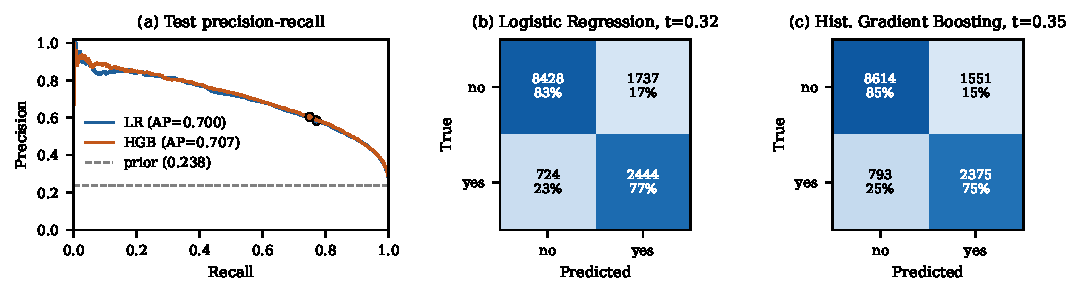
\includegraphics[width=\linewidth]{fig_results.pdf}
\caption{Held-out test set. (a) Precision--recall curves; dots mark the out-of-fold-tuned operating points, the dashed line the prior. (b, c) Confusion matrices at the tuned thresholds (counts and row-normalised rates).}\label{fig:results}\end{figure}

Both models far exceed the prior (AP 0.238). HGB is ahead on the threshold-free metrics: the test AP difference is +0.007 (bootstrap $p$=0.022), consistent with CV (+0.011, corrected $t$-test $p$=0.031). At the tuned thresholds the classifiers disagree on 220\,+\,337 test rows and HGB is right on 337 of them (McNemar $p$ $<$0.001), yet positive-class F1 (CI -0.001 to +0.010) and balanced accuracy (CI -0.006 to +0.003) are statistically tied: HGB's edge lies in ranking, not at the chosen operating point, and is practically small (about one AP point). Threshold tuning matters more than the model: moving LR from 0.5 to 0.32 raises test F1 from 0.624 to 0.665 by trading precision (0.696$\to$0.585) for recall (0.566$\to$0.771); at the tuned thresholds LR misses 724 and HGB 793 of 3{,}168 test positives (Fig.~\ref{fig:results}), at the cost of more false alarms.
\begin{table}[!htb]\centering\footnotesize\setlength{\tabcolsep}{3pt}
\caption{Ablations: one decision reversed, tuned hyper-parameters kept (so $\Delta$ is conservative for the variant). $\Delta$ = change in CV average\_precision on the same folds; sd = sd of paired fold differences ($|\Delta|<$ sd: no detectable effect); $p$: Nadeau--Bengio corrected $t$-test.}\label{tab:ablation}
\begin{tabularx}{\linewidth}{l Y r r r}\toprule
ID & Question & $\Delta$ average\_precision & sd & $p$\\\midrule
A1\_lr\_keep\_zeros & LR: keep co-occurring zeros as values (no NaN + indicator) & +0.0002 & 0.0003 & 0.274\\
A2\_hgb\_keep\_zeros & HGB: keep co-occurring zeros as values (no NaN + indicator) & +0.0004 & 0.0008 & 0.454\\
A3\_lr\_no\_clip & LR: no winsorising of heavy tails & -0.0006 & 0.0004 & 0.093\\
A4\_lr\_keep\_composite & LR: keep the collinear composite\_rank & 0.0000 & 0.0000 & 0.788\\
A5\_hgb\_drop\_composite & HGB: drop composite\_rank & +0.0002 & 0.0015 & 0.821\\
A6\_hgb\_onehot & HGB: one-hot instead of native categorical splits & -0.0035 & 0.0009 & 0.005\\
\bottomrule\end{tabularx}\end{table}


\section{Findings and discussion}
\textbf{(1) The signal appears largely additive.} A linear model on one-hot features comes within about one AP point of boosting, so interactions and non-linear thresholds add little here (with the caveat that the two pipelines also differ in preprocessing). \textbf{(2) Few preprocessing decisions mattered.} Reverting native categorical splits to one-hot changed HGB AP by -0.0035 (A6, $p$=0.005); removing LR's winsorising changed AP by -0.0006 (A3: beyond fold noise but $p$=0.093, weak evidence); zero handling (A1, A2) and the \texttt{composite\_rank} choice (A4, A5) changed AP by less than the fold-to-fold noise. The plan predicted that HGB would profit from \texttt{composite\_rank}; the ablation does not support this, even though permutation importance ranks it second for HGB (0.054). Its information is shared with \texttt{aptitude\_score} and \texttt{performance\_score}: important is not the same as necessary. \textbf{(3) The models read the data differently.} LR leans on \texttt{stability\_index} (importance 0.259), whereas HGB spreads importance over categoricals (\texttt{personal\_interest}, \texttt{instrument}); \texttt{geological\_era}, \texttt{load\_ratio} and \texttt{index\_weight} contribute nothing to HGB.
\textbf{Limitations.} One train/test split; thresholds chosen on the folds that chose hyper-parameters (mildly optimistic); F1 is arbitrary without error costs; anonymised features rule out a domain check of the zero blocks. \textbf{Next steps:} LR with spline features, to separate non-linear main effects from interactions, and a cost-based threshold once costs are known. \textbf{Recommendation:} if transparency matters, LR gives up little; otherwise HGB, tuned to the operating point the application needs.

\FloatBarrier
\label{endofreport}
\clearpage
\section*{Reflection {\normalfont\small(not counted toward the two-page limit)}}
\textbf{Human oversight.} I stayed in the loop mainly by \emph{designing the constraints} rather than by watching each step. Before any code existed I settled, in three question rounds with the agent, the decisions that define the skill: Variant~2; a hybrid design in which deterministic scripts compute every number and the LLM only decides and argues; exactly two contrasting models plus a prior baseline; CV-only model selection with a single use of the test set; AP and macro-F1 as primary metrics; and generalisation tests on two other datasets. I delegated both checkpoints (plan, report) to \emph{fresh} reviewer sub-agents that saw only the files, never the author's reasoning, and required every point and its resolution to be logged (\texttt{runs/in6227/oversight\_log.md}). Those reviews changed the run. The plan review added a missing ablation (zero handling for HGB) and showed that ablation deltas were measured against a selection-biased reference; the skill now reports the sd of paired fold differences and treats $|\Delta|<$ sd as ``no effect''. The report review caught a false sentence (``both models miss under a quarter of positives''; HGB misses 25.03\%) and two over-claims. I also changed the skill itself when it failed: the page check passed while a figure had silently floated to page~3, so it now compiles the main report separately and reads the page count from LaTeX.
\emph{What I would change.} Delegated review is not human review. Next time I would approve the plan myself at checkpoint~1, because that is where the judgement calls are (e.g.\ how to read the zero blocks). I would also freeze the plan and ablation list before the first full run: while the scripts were being debugged, one smoke run printed test metrics. This is disclosed in the log, and no decision traces to it, but a clean protocol would not allow it to happen.

\textbf{Critical evaluation.} The decision I find most questionable is treating the co-occurring zeros as missing (0$\to$NaN plus indicator). The skill argued that zeros shared by several continuous measures mark a structurally different group; that is plausible, but the evidence cuts both ways. (i) The ablations show no benefit for either model ($\Delta$ = +0.0002 and +0.0004, both within fold noise), so the transformation adds complexity for nothing measurable. (ii) The 265-row block is 100\% negative. If those zeros are recorded \emph{after} the outcome, the indicator is a leakage channel; if they mean ``no activity'', it is a legitimate rule. With anonymised features the skill cannot tell the two apart, yet it turned an unresolved semantic question into a confident preprocessing step. I would have kept the raw zeros (simpler, equally accurate) and escalated the block to a human as a data question. A second questionable choice was keeping \texttt{composite\_rank} for HGB on the grounds that trees cannot form linear combinations. The ablation refuted this ($\Delta$ = +0.0002). I agree with how the report handled it: it states the refuted prediction instead of hiding it.

\textbf{Trustworthiness.} Three layers. (1) \emph{By construction}: prose numbers are tokens resolved from \texttt{results.json}, \texttt{profile.json} and \texttt{plan.json}; tables are generated from \texttt{results.json}; unresolved tokens abort the render; every literal typed in the prose is listed in \texttt{numbers\_audit.md}. (2) \emph{Independent review}: the reviewer agent re-derived the HGB tuned-threshold precision, recall, F1 and balanced accuracy, the LR CV AP mean$\pm$sd, the baseline macro-F1 and every ablation sd, and found no mismatch. (3) \emph{Manual check outside the pipeline}: with plain pandas on the raw CSV files I recomputed the labelled row counts (31{,}109 / 13{,}333), the positive share (0.2399) and the 265-row all-negative zero block. I confirmed that \texttt{composite\_rank} $- (0.006\,\texttt{aptitude\_score} + 0.004\,\texttt{performance\_score})$ never exceeds $5\times10^{-4}$ in absolute value, and that HGB's reported recall 0.7497 equals 2375/3168 from its confusion matrix. The one error found, the ``under a quarter'' sentence, was the only claim written as an inference in prose rather than as a token. That is the lesson: the token mechanism protects numbers, not the conclusions drawn from them, so conclusions still need a human or adversarial reader. Finally, generality was tested rather than asserted: the skill was run on two very different datasets (\texttt{examples/}: numeric binary without a test file; categorical 4-class). Those runs exposed two over-sensitive detectors (one flag per correlated pair; KS drift firing on a 114-row hold-out), which I fixed. All three reports were then regenerated with the same final code.

\end{document}
